\documentclass[12pt, twoside]{article}
\usepackage[letterpaper, margin=1in, headsep=0.5in]{geometry}
\usepackage[english]{babel}
\usepackage[utf8]{inputenc}
\usepackage{amsmath}
\usepackage{amsfonts}
\usepackage{amssymb}
\usepackage{tikz}
\usetikzlibrary{quotes, angles}
\usepackage{graphicx}
%\usepackage{pgfplots}
%\pgfplotsset{width=10cm,compat=1.9}
%\usepgfplotslibrary{statistics}
%\usepackage{pgfplotstable}
%\usepackage{tkz-fct}
%\usepackage{venndiagram}
\usepackage{enumitem}
\usepackage{multicol}


\usepackage{fancyhdr}
\pagestyle{fancy}
\fancyhf{}
\fancyhead[LE]{\thepage}
\fancyhead[RO]{%\thepage \\
    Name: \hspace{4cm} \,\\}
\fancyhead[LO]{BECA / Dr. Huson / Geometry 10th Grade\\* Unit 11: Algebra II introduction \\ 4 May 2020}

\renewcommand{\headrulewidth}{0pt}

\begin{document}
\subsubsection*{11.4 Homework: Cosine and sine trigonometry ratios}

\begin{enumerate}

\subsubsection*{Identify each given side of the triangle}
\item $\triangle ABC$ is shown with $m\angle C=90^\circ$ and the triangle's sides are $\overline{AB}$, $\overline{BC}$, and $\overline{AC}$.
  \begin{multicols}{2}
    \begin{enumerate}[itemsep=1cm]
      \item The hypotenuse.
      \item The leg adjacent to $\angle A$.
      \item The side opposite $\angle A$.
    \end{enumerate}
        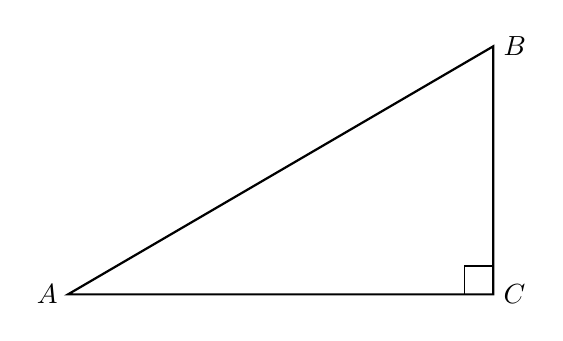
\begin{tikzpicture}[scale=0.9]
          \draw [thick]
          (0,0)node[left]{$A$}--
          (6,0)node[ right]{$C$}--
          (6,3.5)node[right]{$B$}--cycle;
          \draw (6,0)++(-0.4,0)--++(0,0.4)--+(0.4,0);
          %\node at (3,0)[below]{$15$};
          %\node at (6,2)[right]{$8$};
          %\node at (3,2.2)[above]{$17$};
        \end{tikzpicture}
    \end{multicols} \vspace{0.5cm}

\item $\triangle JKL$ is shown with $\overline{JL} \perp \overline{KL}$
  \begin{multicols}{2}
    \begin{enumerate}[itemsep=0.8cm]
      \item The leg opposite $\angle K$.
      \item The side adjacent to $\angle J$.
      \item The hypotenuse.
      \item The leg adjacent to $\angle K$.
      \item The side opposite to $\angle J$.
    \end{enumerate}
        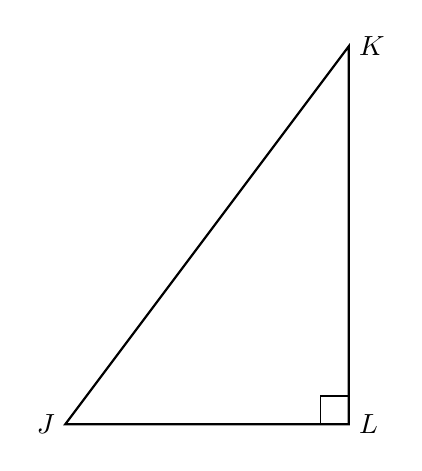
\begin{tikzpicture}[scale=0.6]
          \draw [thick]
          (0,0)node[left]{$J$}--
          (6,0)node[ right]{$L$}--
          (6,8)node[right]{$K$}--cycle;
          \draw (6,0)++(-0.6,0)--++(0,0.6)--+(0.6,0);
          %\node at (3,0)[below]{$15$};
          %\node at (6,2)[right]{$8$};
          %\node at (3,2.2)[above]{$17$};
        \end{tikzpicture}
    \end{multicols} \vspace{0.5cm}
  
\subsubsection*{Write down each value as a ratio (fraction)}

  \item A right $\triangle PQR$ is shown with side lengths 8, 15, and 17, as marked. \vspace{0.5cm}
  \begin{multicols}{2}
    \begin{enumerate}[itemsep=1cm]
      \item $\tan P=$
      \item $\cos P=$
      \item $\sin Q=$
    \end{enumerate}
        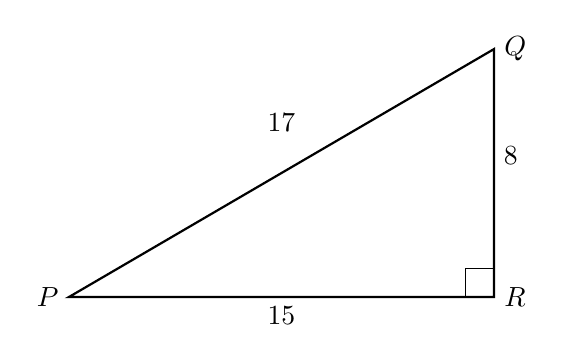
\begin{tikzpicture}[scale=0.9]
          \draw [thick]
          (0,0)node[left]{$P$}--
          (6,0)node[ right]{$R$}--
          (6,3.5)node[right]{$Q$}--cycle;
          \draw (6,0)++(-0.4,0)--++(0,0.4)--+(0.4,0);
          \node at (3,0)[below]{$15$};
          \node at (6,2)[right]{$8$};
          \node at (3,2.2)[above]{$17$};
        \end{tikzpicture}
    \end{multicols}

\end{enumerate}
\end{document}

